\subsection{Clustering}
    Technique that tries to divide the dataset into clusters (groups) that maximize:
    \begin{itemize}
        \item Cohesion: homogeneity within a cluster 
        \item Separation: heterogeneity between clusters 
    \end{itemize}
    Each cluster should contain elements very similar between them and very different from other groups' elements.
    \subsubsection{Clustering for fraud detection}
        We want to detect frauds as deviation from the norm. Frauds can be seen as elements inside the corpus which do not belong to any cluster, or that belong to very small clusters far away from the others.\\
        \textbf{Important:} we're not 100\% sure that them are frauds, they're just outliers, so they need to be investigated to understand what they are.\\ 
        An efficient unsupervised algorithm tries to minimize as much as possible the number of false positives
        \begin{figure}[ht!]
            \centering
            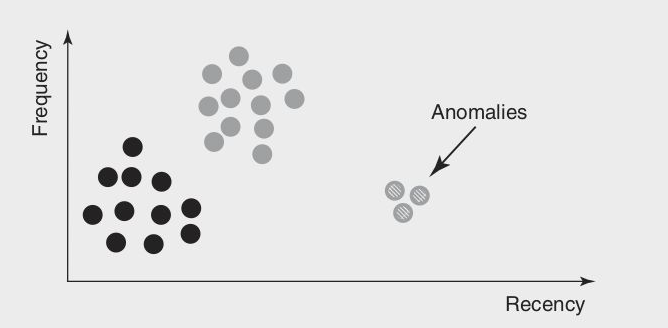
\includegraphics[width=0.6\linewidth]{lecture_13/anomalies.png}
        \end{figure}
    \subsubsection{Distance metric}
        To group elements toghether we need to define a similarity measure:\\
        at the end of the day each element of the cluster must be transformed in vectors of numbers, to understand if two entities are similar we need to compute distance between them.\\
        Possible distance measures can be: euclidean, minkowski or manhattan, mahalanobis \textit{(when high variance in dataset)}
    \subsubsection{Distance metric: Continous vs Categorical}
        \begin{itemize}
            \item \textbf{Continous Variables:}
            \begin{itemize}
                \item Euclidean metric 
                \item Pearson correlation or cosine measure
            \end{itemize}
            \item \textbf{Categorical Variables:} (binary variables 01010101)
            \begin{itemize}
                \item Simple matching coefficient:\\ compute the number of identical matches between the variable values
                \item Jaccard index: measure the similarity between both claims across those red flags raised at least once
            \end{itemize}
        \end{itemize}
\subsection{Clustering Techniques: Hierarchical clustering}
    Two main strategies: \textbf{agglomerative vs divisive}.
    \begin{itemize}
        \item \textbf{Agglomerative strategies:} assign each single element to a cluster, then agglomerate small clusters in greater ones
        \item \textbf{Divisive strategies:} split a great cluster in smaller clusters until each element is assigned to a single cluster
    \end{itemize}
    The final result is usually in between of the two extremes. But to agglomerate/divide, how to compute the distance between clusters?
    \begin{itemize}
        \item \textbf{Single Linkage:} consider the distance between the closest elements in the two clusters 
        \item \textbf{Complete Linkage:} consider the distance between the furthest elements in the two clusters
        \item \textbf{Average Linkage:} consider the average distance between all elements of the two clusters
        \item \textbf{Centroid Method:} elect an element as the representative of the cluster (centroid), compute the distances between centroids
    \end{itemize}
    \subsubsection{Number of Clusters}
        To decide the optimal number of clusters:
        \begin{itemize}
            \item \textbf{Dendrogram:} tree-like diagram that records the sequences of merges. Cut the dendrogram at the desired level to find the optimal clustering
            \item \textbf{Screen Plot:} plot the distance at which clusters are merged, the optimal clustering is indicated by the elbow point
        \end{itemize}
        \begin{figure}[ht!]
            \centering
            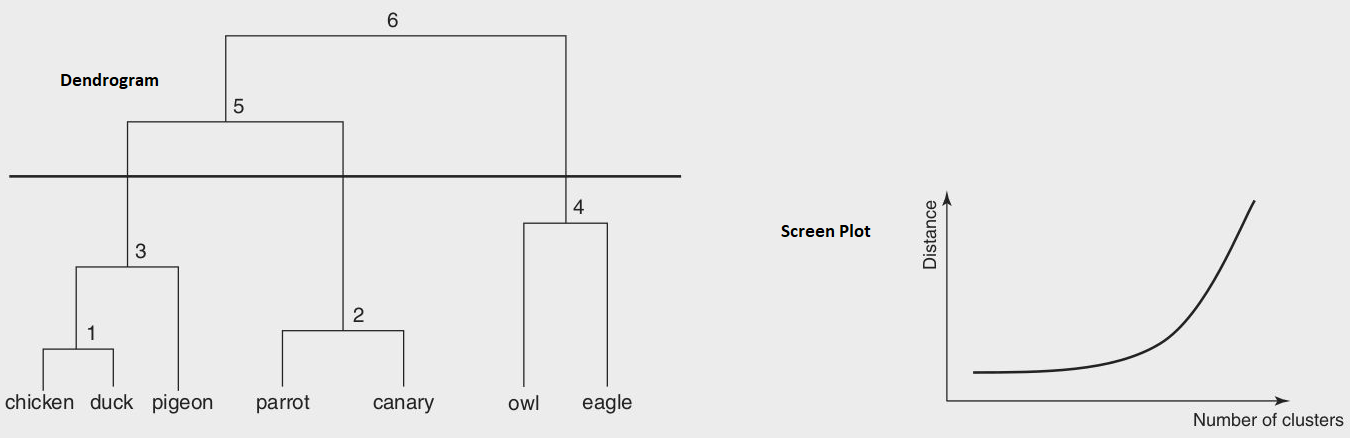
\includegraphics[width=0.6\linewidth]{lecture_13/dendro.png}
        \end{figure}
    \subsubsection{Hierarchical clustering: conclusions}
        \begin{itemize}
            \item \textbf{Advantages:}
            \begin{itemize}
                \item The number of cluster doesn't need to be specified prior to the analysis
            \end{itemize}
            \item \textbf{Disadvantages:}
            \begin{itemize}
                \item Do not scale well to large datasets
                \item The interpretation of the clusters is often subjective and depends on the business expert
            \end{itemize}
        \end{itemize}
\subsection{Clustering Techniques: Non-hierarchical clustering}
    \subsubsection{K-means}
        \begin{itemize}
            \item Select the number of clusters k
            \item Select k observations as initial cluster centroids
            \item Assign each observation to the cluster with the closest centroid according to some distance 
            \item When all observations have been assigned, recalculate the centroids
            \item Repeat until the cluster centroids no longer change
        \end{itemize}
        \textbf{Limitations:}
        \begin{itemize}
            \item The number of cluster must be specified before the start of the analysis, it can be choose by experts or computed as result of other clustering techniques
            \item It is sensitive to outliers, relevant in fraud detection setting
        \end{itemize}
        \begin{figure}[ht!]
            \centering
            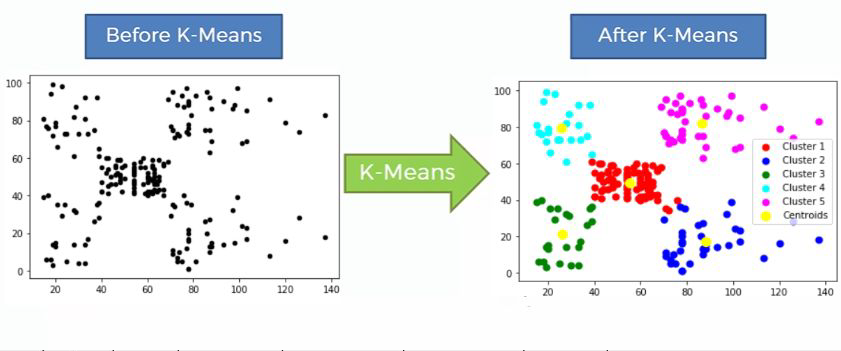
\includegraphics[width=0.6\linewidth]{lecture_13/kmeans.png}
        \end{figure}
    \subsubsection{SOM: Self Organizing Maps}
        It is an unsupervised learning algorithm that allows to visualize and cluster high-dimensional data on low dimensional grids of neurons:\\
        It is a feedforward neural network with an input and an output layer.\\
        Each input is connected to all neurons in output layer with weights, all randomly initialized.\\
        \textbf{Functioning:}\\
        When a training vector x is presented, the weight vector of each neuron is compared with x. The most similar neuron in euclidean sense is called the \textit{BMU: best matching unit}.\\
        Then update all the weights based on BMU: move them towards the point, trying so to match the distribution of the original points.
        \begin{itemize}
            \item \textbf{Advantages:} it is able to automatically cluster data, results can be visualized and interpreted
        \end{itemize}